\section*{\huge \textcolor{Red}{Data Efficient Learning}  \small \textit{??? chưa dịch ???} }
Tham khảo\footnote{https://arxiv.org/abs/2102.12903} (tạm để đây, còn khi dịch sau sẽ xoá hoặc giấu dòng này đi)
\subsection*{Định nghĩa:}
???
\subsection*{Ví dụ:}
???
\subsection*{Mẹo nhỏ:}
???
%%
\section*{\huge \textcolor{Red}{Dark data}  \small \textit{??? chưa dịch ???} }
Tham khảo\footnote{https://www.bmc.com/blogs/dark-data/} (tạm để đây, còn khi dịch sau sẽ xoá hoặc giấu dòng này đi)
\subsection*{Định nghĩa:}
???
\subsection*{Ví dụ:}
???
\subsection*{Mẹo nhỏ:}
???
%%
\section*{\huge \textcolor{Red}{Deep Reinforcement Learning}  \small \textit{??? chưa dịch ???} }
Tham khảo\footnote{} (tạm để đây, còn khi dịch sau sẽ xoá hoặc giấu dòng này đi)
\subsection*{Định nghĩa:}
???
\subsection*{Ví dụ:}
???
\subsection*{Mẹo nhỏ:}
???
%%
\section*{\huge \textcolor{Red}{Decision Support System}  \small \textit{??? chưa dịch ???} }
Tham khảo\footnote{} (tạm để đây, còn khi dịch sau sẽ xoá hoặc giấu dòng này đi)
\subsection*{Định nghĩa:}
???
\subsection*{Ví dụ:}
???
\subsection*{Mẹo nhỏ:}
???
%%
\section*{\huge \textcolor{Red}{Distributed Artificial Intelligence}  \small \textit{??? chưa dịch ???} }
Tham khảo\footnote{} (tạm để đây, còn khi dịch sau sẽ xoá hoặc giấu dòng này đi)
\subsection*{Định nghĩa:}
???
\subsection*{Ví dụ:}
???
\subsection*{Mẹo nhỏ:}
???
%%
\section*{\huge \textcolor{Red}{Description Logic}  \small \textit{??? chưa dịch ???} }
Tham khảo\footnote{} (tạm để đây, còn khi dịch sau sẽ xoá hoặc giấu dòng này đi)
\subsection*{Định nghĩa:}
???
\subsection*{Ví dụ:}
???
\subsection*{Mẹo nhỏ:}
???
%%
\section*{\huge \textcolor{Red}{Descriptive Statistics}  \small \textit{??? chưa dịch ???} }
Tham khảo\footnote{https://deepai.org/machine-learning-glossary-and-terms/descriptive-statistics} (tạm để đây, còn khi dịch sau sẽ xoá hoặc giấu dòng này đi)
\subsection*{Định nghĩa:}
???
\subsection*{Ví dụ:}
???
\subsection*{Mẹo nhỏ:}
???
%%
\section*{\huge \textcolor{Red}{Decision Boundary}  \small \textit{Ranh giới quyết định} }
Tham khảo\footnote{\url{https://en.wikipedia.org/wiki/Decision_boundary}}
\subsection*{Định nghĩa:}
Trong bài toán phân loại, \textbf{Ranh giới quyết định} là đường, mặt phẳng, hay siêu mặt phẳng giúp phân chia vùng của các cụm (cluster) dữ liệu trong không gian.
Bộ phân loại sẽ coi các điểm nằm cùng 1 phía của ranh giới quyết định cùng thuộc 1 lớp, và các điểm nằm về phía còn lại của ranh giới cùng thuộc lớp còn lại.

Trong học máy, ranh giới quyết định tồn tại dưới nhiều dạng khác nhau.
Trong mạng nơ-ron nhân tạo, nếu mạng không có tầng ẩn nào thì mạng chỉ có thể học ranh giới tuyến tính, còn nếu mạng có ít nhất một tầng ẩn thì mạng có thể học bất kì dạng ranh giới nào (theo Universal approximation theorem).
\subsection*{Ví dụ:}
\begin{figure*}[!h]
    \centering
    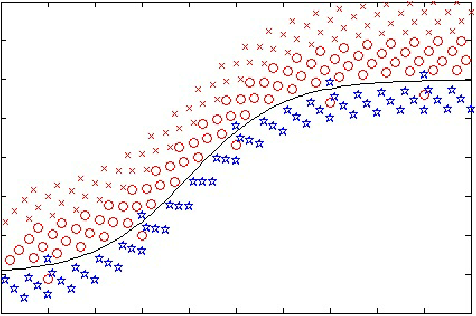
\includegraphics[width=1.0\linewidth]{figures/D_Decision_boundary.png}
    \caption{Ranh giới quyết định. Các điểm ở phía trên ranh giới cùng thuộc 1 lớp (màu đỏ), trong khi đó các điểm nằm phía dưới ranh giới thuộc lớp còn lại (màu xanh).}
    \label{fig:D_Decision_boundary}
\end{figure*}
% \subsection*{Mẹo nhỏ:}
%%
\section*{\huge \textcolor{Red}{Decision Tree}  \small \textit{??? chưa dịch ???} }
Tham khảo\footnote{https://developers.google.com/machine-learning/glossary\#decision-tree} (tạm để đây, còn khi dịch sau sẽ xoá hoặc giấu dòng này đi)
\subsection*{Định nghĩa:}
???
\subsection*{Ví dụ:}
???
\subsection*{Mẹo nhỏ:}
???
%%
\section*{\huge \textcolor{Red}{Deductive Reasoning}  \small \textit{??? chưa dịch ???} }
Tham khảo\footnote{https://towardsdatascience.com/the-paradox-of-deductive-reason-in-data-science-featuring-donald-trumps-twitter-account-43839d4dda82} (tạm để đây, còn khi dịch sau sẽ xoá hoặc giấu dòng này đi)
\subsection*{Định nghĩa:}
???
\subsection*{Ví dụ:}
???
\subsection*{Mẹo nhỏ:}
???
%%
\section*{\huge \textcolor{Red}{Discrete Random Variable}  \small \textit{??? chưa dịch ???} }
Tham khảo\footnote{https://deepai.org/machine-learning-glossary-and-terms/discrete-random-variable} (tạm để đây, còn khi dịch sau sẽ xoá hoặc giấu dòng này đi)
\subsection*{Định nghĩa:}
???
\subsection*{Ví dụ:}
???
\subsection*{Mẹo nhỏ:}
???
%%
\section*{\huge \textcolor{Red}{Deep Belief Network}  \small \textit{??? chưa dịch ???} }
Tham khảo\footnote{http://www.wildml.com/deep-learning-glossary/\#rnn} (tạm để đây, còn khi dịch sau sẽ xoá hoặc giấu dòng này đi)
\subsection*{Định nghĩa:}
???
\subsection*{Ví dụ:}
???
\subsection*{Mẹo nhỏ:}
???
%%
\section*{\huge \textcolor{Red}{Denoising Autoencoders}  \small \textit{??? chưa dịch ???} }
Tham khảo\footnote{https://deepai.org/machine-learning-glossary-and-terms/denoising-autoencoder} (tạm để đây, còn khi dịch sau sẽ xoá hoặc giấu dòng này đi)
\subsection*{Định nghĩa:}
???
\subsection*{Ví dụ:}
???
\subsection*{Mẹo nhỏ:}
???
%%
\section*{\huge \textcolor{Red}{Dropout Regularization}  \small \textit{??? chưa dịch ???} }
Tham khảo\footnote{https://medium.com/analytics-vidhya/a-simple-introduction-to-dropout-regularization-with-code-5279489dda1e} (tạm để đây, còn khi dịch sau sẽ xoá hoặc giấu dòng này đi)
\subsection*{Định nghĩa:}
???
\subsection*{Ví dụ:}
???
\subsection*{Mẹo nhỏ:}
???
%%
% \section*{\huge \textcolor{Red}{}  \small \textit{??? chưa dịch ???} }
% Tham khảo\footnote{} (tạm để đây, còn khi dịch sau sẽ xoá hoặc giấu dòng này đi)
% \subsection*{Định nghĩa:}
% ???
% \subsection*{Ví dụ:}
% ???
% \subsection*{Mẹo nhỏ:}
% ???
% %%